\chapter{Stream Processing Platforms}
In practice, there are plenty of cases that need stable and efficient stream processing system to deal with continuously incoming data. In some case, results of data processing could be required in minutes or even in seconds. Such as sensors data should be processed and monitored on the dashboard as soon as possible. Examples of stream processing systems include Apache Apex, Aurora, S4, Storm, Samza, Flink, Spark Streaming, IBM InfoSphere Streams, Amazon Kinesis and many others. The design and architecture of these systems are different so that they own different features. Three open source systems: Storm, Flink and Spark which are widely used in a range of applications are choose in our benchmark. As these are open source systems, it is possible to set up our own distribute cluster to run experiment benchmarks. 

In this chapter, we will introduce these three systems in detail from different perspectives: system architecture, core concepts and key features. Several other stream processing systems are also discussed. 
 
\section{Apache Storm}
Apache Storm, one of oldest distributed stream processing system which was open sourced by Twitter in 2011 and became Apache top-level project in 2014.  Storm is to realtime data processing as Apache Hadoop and MapReduce are to batch data processing. Storm solutions can also provide guaranteed processing of data, with the ability to replay data that was not successfully processed the first time.With its simple programming interface, Storm allows application developers to write applications that analyze streams of tuples of data; a tuple may can contain object of any type.

\subsection{Storm Architecture}
\begin{figure}
  \begin{center}
  \subfigure{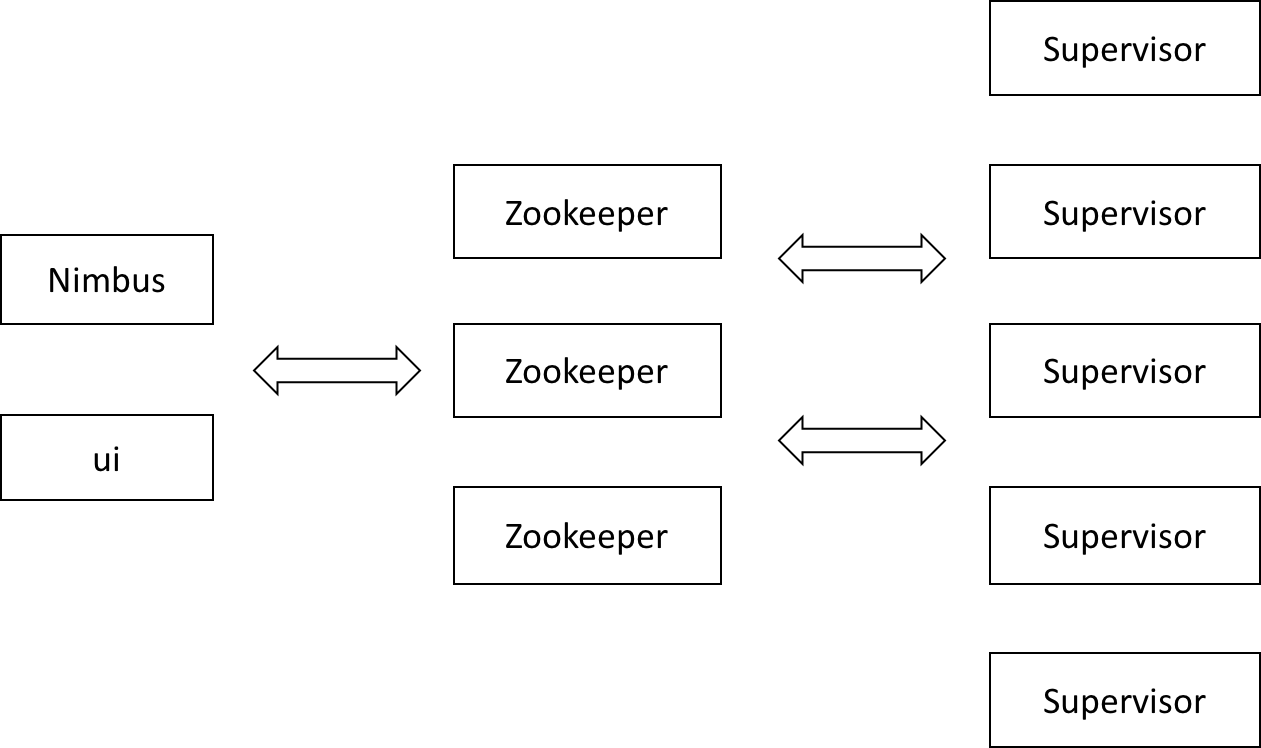
\includegraphics[scale=0.5]{images/storm_cluster}}
   \caption{Storm cluster components}
   \label{fig:storm_cluster}
  \end{center}
\end{figure}

As a distributed stream processing system, a storm cluster consists of a set of nodes. Figure~\ref{fig:storm_cluster} shows components of a storm cluster which contains four different kinds of nodes, "Supervisor", "Nimbus", "Zookeeper" and "ui". 

"Nimbus" is a daemon runs on the master node which is similar to Hadoop's "JobTracker". Nimbus is responsible for distributing code around the cluster, assigning tasks to machines, and monitoring for failures. Each worker node runs a daemon called the "Supervisor." It listens for work assigned to its machine and starts and stops worker processes as dictated by Nimbus. Each worker process executes a subset of a topology; a running topology consists of many worker processes spread across many machines.

All coordination between Nimbus and the Supervisors is done through a Zookeeper cluster. Additionally, the Nimbus daemon and Supervisor daemons are fail-fast and stateless; all state is kept in Zookeeper or on local disk. This means you can kill -9 Nimbus or the Supervisors and they'll start back up like nothing happened. Hence, Storm clusters are stable and fault-tolerant

"ui" is a daemon which monitors summary of cluster and running topologies on a web interface. The summary of cluster includes storm version, Nimbus up-time, the number of Supervisors, etc. Properties of a topology (such as id, name, status and uptime) and emitted tuples of a spout/bolt also could be found in "ui". More detail about understanding the Storm UI could be found on the page~\footnote{\url{http://www.malinga.me/reading-and-understanding-the-storm-ui-storm-ui-explained/}}.


\subsection{Computing Model}

At the core of Storm's data stream processing is a computational topology,  which is a graph of stream transformations where each node is a spout or bolt. Edges in the graph indicate which bolts are subscribing to which streams as shown in Figure~\ref{fig:storm_model}.

Spouts are the sources of streams in a topology which will read tuples from external sources (e.g. Twitter API, Kafka) or from disk and emit them in the topology. Bolt receives input streams from spout or other bolt, process them and produce output streams. They encapsulate the application logic which dictates how tuples are processed, transformed,aggregated, stored, or re-emitted to other nodes in the topology for further processing. When a spout or bolt emits a tuple to a stream, it sends the tuple to every bolt that subscribed to that stream.

A stream in topology is an unbounded sequence of tuples. Spouts read tuples from external sources continuously. Once a topology is submitted, it processes messages forever, or until it is killed. Storm will automatically reassign any failed tasks. Additionally, Storm guarantees that there will be no data loss, even if machines go down and messages are dropped.

Each node in a Storm topology executes in parallel. In your topology, you can specify how much parallelism you want for each node, and then Storm will spawn that number of threads across the cluster to do the execution.

Guaranteed processing

\begin{figure}
  \begin{center}
  \subfigure{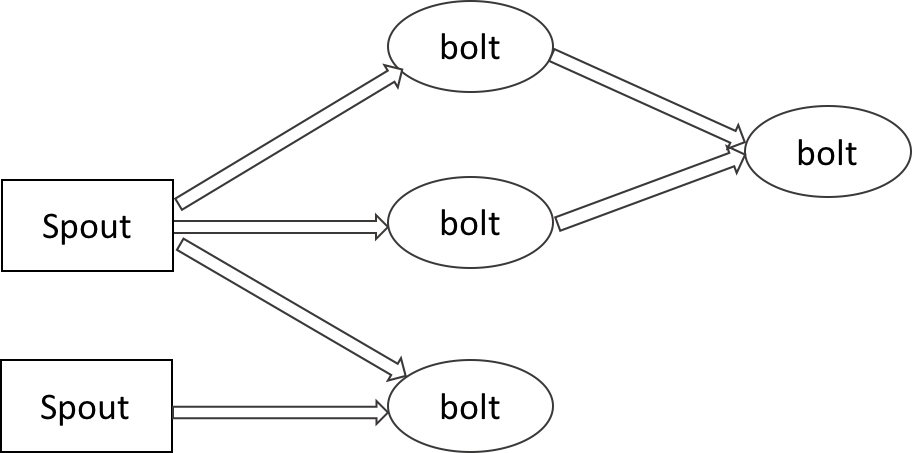
\includegraphics[scale=0.7]{images/storm_model}}
   \caption{Storm topology model}
   \label{fig:storm_model}
  \end{center}
\end{figure}

\section{Apache Flink}
Apache Flink used to be known as Stratosphere which was started off as an academic open source project in Berlin's Technical University in 2010. Later, it became a part of the Apache Software Foundation incubator and was accepted as an Apache top-level project in December 2014. Apache Flink aims to be a next generation system for big data system. It is a replacement for Hadoop MapReduce that works in both batch and streaming models. Its defining feature is its ability to process streaming data in real time. In Flink, batch processing applications run efficiently as special cases of stream processing applications.

\subsection{Flink Architecture}
The architecture of Flink is a typical master-slave architecture that is quite similar with other scaleable distribute cloud systems. The system consists of a JobManager and one or more TaskManagers. The JobManager is the coordinator of the Flink system, while the TaskManagers are the workers that execute parts of the parallel programs. 

In Hadoop MapReduce, a operation wouldn't start until the previous operation is finished. In Flink records are forwarded to receiving tasks as soon as they are produced which is called pipelined data transfers. For efficiency, these records are collected in a buffer which is sent over the network once it is full or a certain time threshold is met. This threshold controls the latency of records because it specifies the maximum amount of time that a record will stay in a buffer without being sent to the next task. 

Flink's runtime natively supports both domains due to pipelined data transfers between parallel tasks which includes pipelined shuffles. Batch jobs can be optionally executed using blocking data transfers. They are special cases of stream processing applications.

\subsection{Memory Management}
One specific feature of Flink is that Flink has its own memory management system. Conceptually, Flink splits the heap into three regions: ~\footnote{\url{https://cwiki.apache.org/confluence/pages/viewpage.action?pageId=53741525}}

\begin{itemize}
\item \textbf{Network buffers:} A number of 32 KiByte buffers used by the network stack to buffer records for network transfer. Allocated on TaskManager startup. 
\item \textbf{Memory Manager pool:} A large collection of buffers (32 KiBytes) that are used by all runtime algorithms whenever they need to buffer records. Records are stored in serialized form in those blocks.
\item \textbf{Remaining (Free) Heap:} This part of the heap is left to the user code and the TaskManager's data structures.
\end{itemize}
 
In Flink memory management is used for all operations that accumulate a number of records. Without memory management tool, operations would fail when the data is larger than the memory that JVM could spare. The memory management is a way to control very precisely how much memory each operator uses, and to let them de-stage efficiently to out-of-core operation, by moving some of the data do disk. Currently, the memory management is used only in batch operations. 

\section{Apache Spark}
\label{section:spark}

Apache Spark is currently the most actively open source large-scale data processing framework used in many enterprises across the world. It was originally developed in 2009 in UC Berkeley's AMPLab, and open sourced in 2010 as an Apache project. Compared to other big data and MapReduce technologies like Hadoop and Storm, Spark has several advantages. 

Spark is very easy to use by providing APIs in Scala, Java, Python and R languages. Moreover, there are more than 80 high-level built-in operators.  In the case of implementing a simple WordCount application, all the execution logic code could be written in one line with Spark' Scala API.

Spark powers a stack of libraries including SQL and DataFrames, MLlib for machine learning, GraphX, and Spark Streaming. You can combine these libraries seamlessly in the same application. It can access diverse data sources including HDFS, Cassandra, HBase, and S3.

Spark achieves much better performance than Hadoop MapReduce. Spark has an advanced Direct Acyclic Graph(DAG) execution engine that supports cyclic data flow and in-memory computing. By using RDDs which will be discussed in next subsection, intermediate results are stored in memory and reused for further performing functions thereafter, as opposed to being written to hard disk. 

\subsection{ Resilient Distributed Dataset(RDD)}

\textbf{R}esilient \textbf{D}istributed \textbf{D}ataset(RDD) is a fault-tolerant abstraction of read-only collection of elements partitioned across the distributed computer nodes in memory which can be operated on in parallel. RDDs can only be created through deterministic operations on either (1) data in stable storage or (2) other RDDs\cite{zaharia2012resilient}. 

RDD supports two different kinds of operations, transformation and action.  When a transformation operation is called on a RDD object, a new RDD returned and the original RDD remains the same. For example, map is a transformation that passes each element in RDD through a function and returns a new RDD representing the results. Some of the transformation operations are  map, filter, flatMap, groupByKey and reduceByKey. 

An action returns a value to the driver program after running a computation on the RDD. Reduce is an action that aggregates all the elements of the RDD using some function and returns the final result to the driver program.

No matter how an RDD is created, it keeps all information about how it was derived from other dataset to compute its partitions from data in stable storage or how it is transformed from other RDD. Therefore, RDDs are fault tolerance because they could be reconstructed from a failure with these kept information. 

All transformations in Spark are lazy, in that they do not compute their results right away. Instead, they just remember the transformations applied to some base dataset (e.g. a file). The transformations are only computed when an action requires a result to be returned to the driver program. This design enables Spark to run more efficiently ? for example, we can realize that a dataset created through map will be used in a reduce and return only the result of the reduce to the driver, rather than the larger mapped dataset.

By default, each transformed RDD may be recomputed each time you run an action on it. However, by caching RDD in memory, allowing it to be reused efficiently across parallel operations. The recomputation of cached RDD is avoid  and a significant amount of disk I/O could be reduced. Especially in the case of looping jobs, the performance would be improved. In Spark, users can manually specify if working sets are cached or not. The runtime engine would manage low-level caching mechanism like how to distribute cache blocks.

\subsection{Spark Streaming}
\begin{figure}
  \begin{center}
  \subfigure{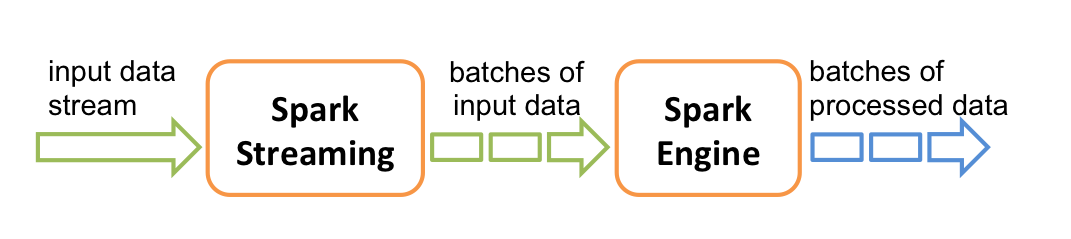
\includegraphics[scale=0.7]{images/spark_stream}}
   \caption{Spark Streaming Model}
   \label{fig:spark_stream}
  \end{center}
\end{figure}

Spark Streaming is an extension of the core Spark API that enables scalable, high-throughput, fault-tolerant stream processing of live data streams. 

Spark Streaming receives live input data streams and divides the data into batches, which are then processed by the Spark engine to generate the final stream of results in batches. The model of Spark Streaming is different from that of Storm and Flink, which process stream records one by one. In Spark Streaming, data streams are divided according to a batch interval which could be configured in the program. Divided data stream is abstracted as discretized stream or DStream, which represents a continuous stream of data. 

DStreams can be created either from input data streams from sources such as Kafka, Flume, and Kinesis, or by applying high-level operations on other DStreams. Internally, a DStream is represented as a sequence of micro RDDs. After applied transformations or actions on a DStream,   a new DStream or result values would be get which can be pushed out to filesystems, databases, and live dashboards.

\section{Other Stream Processing Systems}
\subsection{Apache Samza}
Apache Samza is a top-level project of Apache Software Foundation which open sourced by LinkedIn to solve stream processing requirements. It?s been in production at LinkedIn for several years and currently runs on hundreds of machines. 

A Samza application is constructed out of streams and jobs. A stream is composed of immutable sequences of messages of a similar type or category.  A Samza job is code that performs a logical transformation on a set of input streams to append output messages to set of output streams. In order to scale the throughput of the stream processor, streams are are are broken into partitions and jobs are broken into smaller units of execution called tasks. Each task consumes data from one or more partitions for each of the job's input streams. Multiple jobs could be composed together to create a dataflow graph, where the nodes are streams containing data, and the edges are jobs performing transformations. 

\begin{figure}
  \begin{center}
  \subfigure{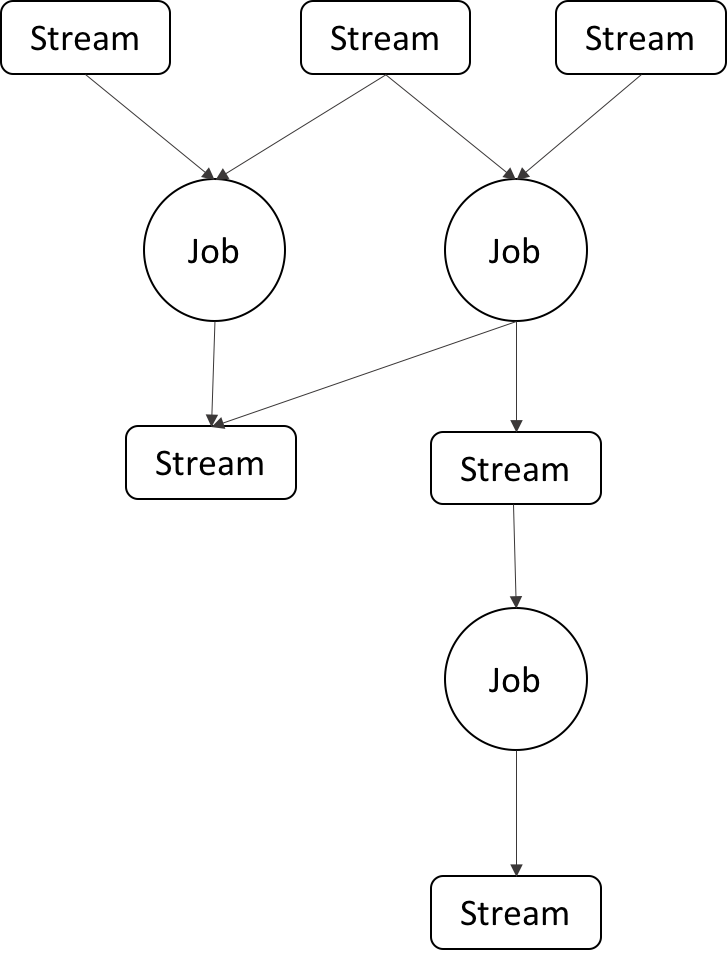
\includegraphics[scale=0.5]{images/samza_dataflow}}
   \caption{Samza DataFlow Graph}
   \label{fig:smaza_dataflow}
  \end{center}
\end{figure}

Except streams and jobs, Samza uses  YARN as execution layer. The architecture of Samza follows a similar pattern to Hadoop which could be shown as Figure~\ref{fig:smaza_architecture}.

\begin{figure}
  \begin{center}
  \subfigure{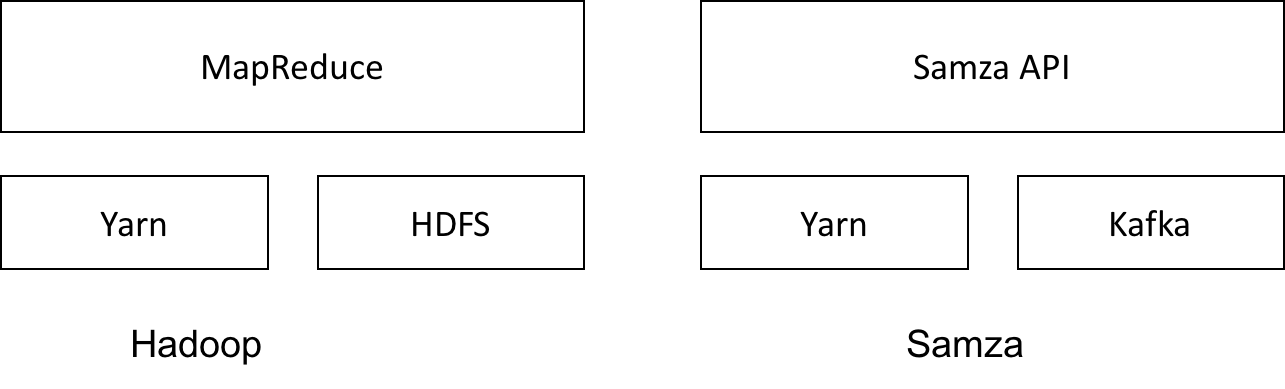
\includegraphics[scale=0.5]{images/samza_architecture}}
   \caption{Samza and Hadoop architecture}
   \label{fig:smaza_architecture}
  \end{center}
\end{figure}

\subsection{Apache S4}
S4 is another open source distributed, scalable, fault-tolerant, stream data processing platform released by Yahoo.

In S4, a stream is defined as a sequence of events of the form (\textbf{K,V}) where \textbf{K} is the key of record tuple, and V is the corresponding value. Processing Element(PE) is the basis computational unit that consume streams and applies computational logic. After takes in an event, a PE either emits one or more events which may be consumed by other PEs or publishes results\cite{neumeyer2010s4}.

S4 makes sure that two events with the same key end up being processed on the same machine. Crucial to the scalability of S4 is the idea that every instance of a processing element handles only one key. The size of an S4 cluster corresponds to the number of logical partitions. 
 
\clearpage